\documentclass[11pt]{article}
\addtolength{\oddsidemargin}{-1.cm}
\addtolength{\textwidth}{2cm}
\addtolength{\topmargin}{-2cm}
\addtolength{\textheight}{3.5cm}
\newcommand\tab[1][1cm]{\hspace*{#1}}
\usepackage[pdftex]{graphicx}
\usepackage{pdflscape}
\usepackage[T1]{fontenc}
\usepackage{hyperref}
\usepackage{float}
\usepackage{cite}
\hypersetup{
	colorlinks=true,
	linkcolor=black,
	filecolor=magenta,
	urlcolor=cyan,
}

% define the title
\author{Panda Inc}
\title{Momentum -- Multiply Active Dayz App}
\begin{document}
\begin{titlepage}
	
	\begin{center}
		% Upper part of the page         
        
\includegraphics[width=0.7\linewidth]{Images/PandaInc_logo.jpg}\\[1cm] 
		\textsc{\LARGE Panda Inc}\\[0.3cm]
		% Title
		\rule{\linewidth}{0.5mm} \\[1cm]
		{ \huge \bfseries Momentum - Multiply Active Dayz App}\\[0.5cm]
		\rule{\linewidth}{0.5mm} \\[1cm] 		
  
		
		\begin{minipage}{0.4\textwidth}
			\begin{flushleft} \large
				\emph{} \\
				Quinton {Swanepoel}
			\end{flushleft}
		\end{minipage}
		\begin{minipage}{0.4\textwidth}
			\begin{flushright} \large
				\emph{} \\
				15245510
			\end{flushright}
		\end{minipage}

		\begin{minipage}{0.4\textwidth}
			\begin{flushleft} \large
            	\emph{} \\
				Azhar {Patel}
			\end{flushleft}
		\end{minipage}
		\begin{minipage}{0.4\textwidth}
			\begin{flushright} \large
				\emph{} \\
				15052592
			\end{flushright}
		\end{minipage}
		
		\begin{minipage}{0.4\textwidth}
			\begin{flushleft} \large
				\emph{} \\
				Tshepo Macebo {Malesela}
			\end{flushleft}
		\end{minipage}
		\begin{minipage}{0.4\textwidth}
			\begin{flushright} \large
				\emph{} \\
				14211582
			\end{flushright}
		\end{minipage}

		\begin{minipage}{0.4\textwidth}
			\begin{flushleft} \large
				\emph{} \\
				Monkeli Fred {Dilapisho}
			\end{flushleft}
		\end{minipage}
		\begin{minipage}{0.4\textwidth}
			\begin{flushright} \large
				\emph{} \\
				15074260
			\end{flushright}
		\end{minipage}
        
        \begin{minipage}{0.4\textwidth}
			\begin{flushleft} \large
				\emph{} \\
				Keaton {Pennels}
			\end{flushleft}
		\end{minipage}
		\begin{minipage}{0.4\textwidth}
			\begin{flushright} \large
				\emph{} \\
				14373018
			\end{flushright}
		\end{minipage}
		
		\rule{\linewidth}{0.5mm} \\[1cm] 
		\textsc{\Large Stakeholders}\\[1cm]	
		
		\begin{minipage}{0.4\textwidth}
			\begin{flushleft} \large
				\emph{} \\
				MMI Holdings:
			\end{flushleft}
		\end{minipage}
		\begin{minipage}{0.4\textwidth}
			\begin{flushright} \large
				\emph{} \\
				Phillip Kruger
			\end{flushright}
		\end{minipage}

		
	\end{center}
\end{titlepage}

\newpage
\tableofcontents
\newpage

\section{Panda Inc.}
\subsection{About Us}
Panda Inc. is a team of hard working passionate software developers. Each member of the team brings their own unique, diverse skill set to the table, which includes competence in a wide range of fields such as Artificial Intelligence, multimedia and also business intellect. Panda Inc. has a fun and modern culture that promotes blue sky thinking and solutions that fit into the modern environment. The team works exceptionally well together and all members aim to produce a quality product while also creating a constructive relationship with our client.


\subsection{The Team}
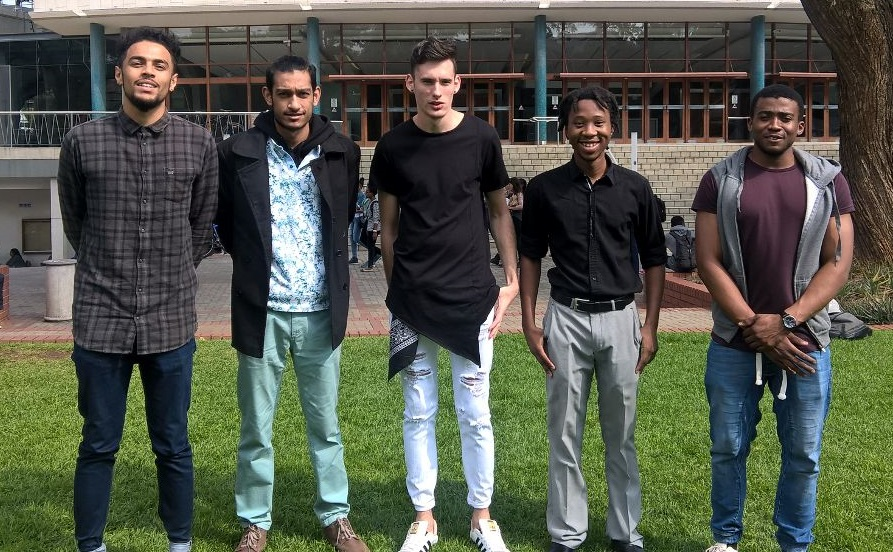
\includegraphics[width=\textwidth]{Images/Team_Pic.jpg}

\subsubsection{Quinton Swanepoel} 
\paragraph{}Course : BSc Computer Science (with Infomratics)
\paragraph{}Career Interest : Software Development / Business Systems Development  
\paragraph{}Skills : 
\begin{itemize}
\item Programming (C++, Java, C\#)
\item Web Development
\item Systems Design
\item Mobile Development (Android Studio, Xamarin)
\end{itemize}
\paragraph{Bio :}I started at the University of Pretoria in 2015 studying computer science, second year I  decided to start taking the prescribed BCom Informatics modules in addition to my computer science modules. This is because I love the business aspect of IT but I'm also interested in the deeper back-end development sector and wish to have as much knowledge as I can about systems development, front-end development, and back-end development which is not all taught in one degree. I am passionate about what I am studying which makes putting in the extra effort to always produce a perfect product that much easier. 

\subsubsection{Azhar Patel}
\paragraph{}Course : BSc Computer Science
\paragraph{}Career Interest : Software/Game Development and Security
\paragraph{}Skills : 
\begin{itemize}
\item Adept in C++ and Java
\item HTML with PHP and JavaScript
\item Mobile Development in Android
\item Artificial Intelligence 
\end{itemize}
\paragraph{Bio :}Currently in my final year at the University of Pretoria having started in 2015. I've enjoyed Psychology as an elective in my first year and it has enhanced my enthusiasm for Psychology in the Computer Science field, hence choosing a Multimedia module that focuses on Human-Computer Interaction along with gaming. Prior to University, I had a great interest in computers and excelled in Mathematics. Computer Science is composed of all of the aforementioned aspects and my passion for the field has grown eversince. I like meeting new people and solving a variety of different problems. I also enjoy online gaming which keeps my mind alert. I am dilligent and will sacrifice sleep if needed. Furthermore, I am a loyal guy and this will be portrayed one day towards the company that employs me. My final goal is to one day help people in need, possibly via programming and applications. We cannot help everyone in the world, but helping a few people can go a long way in helping many in need.

\subsubsection{Tshepo Macebo Malesela}
\paragraph{}Course : BSc Computer Science
\paragraph{}Career Interest : Software Engineering and Component Development
\paragraph{}Skills : 
\begin{itemize}
\item Programmed in C++ and java, the focus was mainly Object-oriented languages.
\item C, mainly at work, with .Net Core, MVC 6 and domain development.
\item HTML, component develepment with polymer and angular.
\item Javascript, for functionality on front-end development.
\item PHP, during my first and second year
\end{itemize}
\paragraph{Bio :} I am a student studying computer science at the University of Pretoria with a strong passion for system development and component development. Before University I believed I was going to study mathematics because at the time I really enjoyed it but by the time I had began my matric year I realised that I had a strong passion for computers, and systems. I am comfortable with front-end and back-end development. Being a student and a part-time worker has given me the skill of learning very quickly. I am very friendly, I would describe myself as a peoples person. Communication is very important to me, I honestly believe good communication makes working easier because everyone know where everyone stands. I am beginning to learn and love the business side of software development (i.e the software engineering), because I have learned that in order to make a good software product there is much more than just the good software development that is required to make the application a product. I am still learning and developing my skill as a programmer and I enjoy challanges.

\subsubsection{Monkeli Fred Dilapisho}
\paragraph{}Course : BSc Computer Science
\paragraph{}Career Interest : Software Development
\paragraph{}Skills : 
\begin{itemize}
\item Multimedia - Website Development
\item Proficient in Java and C++ Object Oriented Programming.
\item Artificial Intelligence
\end{itemize}
\paragraph{Bio :}  Having started this degree in 2015, I am a final year student at the University of Pretoria. My interest in computer science is born from IT classes in high school as well as my innate propensity for desconstructing computer technologies if only to understand better how they work. I have a long history of being dedicated to long term projects and my commitment to choral activities at the University of Pretoria is proof of this. I have an unwavering interest in developing artificial intelligence based off of maps of the human brain and find the question of mapping every connection in the human brain to be an interesting and challenging one.

\subsubsection{Keaton Pennels}
\paragraph{}Course : BSc Computer Science 
\paragraph{}Career Interest : Software Engineering, Social Entrepreneurship
\paragraph{}Skills :
\begin{itemize}
\item Programming in Object Oriented Languages such as Java, C++, C
\item Competent in Assembly (Intel)
\item Web Development - Experienced in both the LAMP(Linux, Apache, MySQL, PHP) stack and the MEAN (MongoDB, Eclipse, AngularJS, Node) stack as well as MVC based implementation.
\item Project Management
\end{itemize}
\paragraph{Bio :}I am a second generation Software Engineer, inspired by my mother to pursue a career in Computer Science. I see software engineering as a means to not only engage myself in the technologically driven world we live in, but also as a conduit to producing products and services for the empowerment of the general masses. Software Engineering is a field of work that I am highly passionate about and it is my intention to commit the rest of my life to perfecting skills required to be a stand out operative, with respect to both the programming and engineering aspects of the field.

\section{Motivation For Project}
When deciding what projects to bid for, each team member suggested three projects which they were interested in. The Multiply Active Dayz App is the only project that every team member had a mutual interest in, and was individually suggested by every member. This common interest increases the chances of project success as well as the chance of producing a top-level application as we are all willing to go the extra mile on this project, hence this is our first choice project.
\newline
\newline Every team member also has skills that will contribute to making this a successful project. The team has members who major in multimedia and business, these members will focus on the front-end development of the project and produce an application with a flawless user experience and user interface. The team members focused on data management and AI will work on the back-end of the project. These members will handle server side programming and the analytic algorithms needed, as well as the cloud based service integration. We all have more than sufficient skills to handle the development of the Admin Web Interface due to us sharing similar backgrounds in web development both client and server side. 
\newline
\newline We are the best choice for this project because of our diverse skills and excellent team work. With our common interest in this project we aim at doing our best to meet all the client's requirements and exceed expectations.

\section{The Project}
\subsection{High Level Description}
The project is to develop a mobile application that can determine how long a certain user has been at a certain location. A web interface will be designed for the Admin to manage partners.
\newline
\newline The following requirements will be met : 
\begin{itemize}
\item Ability to see current number of active days on the app.
\item The ability to create a new community
\item The ability to join an existing community
\item The ability to invite friends to join a community
\item The ability to create challenges in a community 
\item The ability for communities to compete against each other on certain challenges
\item Results and challenges should be able to be shared on multiple social media platforms directly from the app.
\item The app should have a community and a global leader board
\item Users should be able to win prizes instantly through winning challenges (Airtime, Data, Vouchers etc)
\item Analytics integration should be done to monitor app usage.
\end{itemize}


\subsection{Technologies To Be Used}
\begin{itemize}
\item Front-end : Java 
\item Back-end : Java / Apache
\item Database : Neo4j (Graph)
\item Cloud Services : Amazon Web Services
\item Container : Docker
\item Location Based Services : Estimote Beacons, Lisnr
\end{itemize}

\subsection{Deployment Diagram}
\begin{center}
 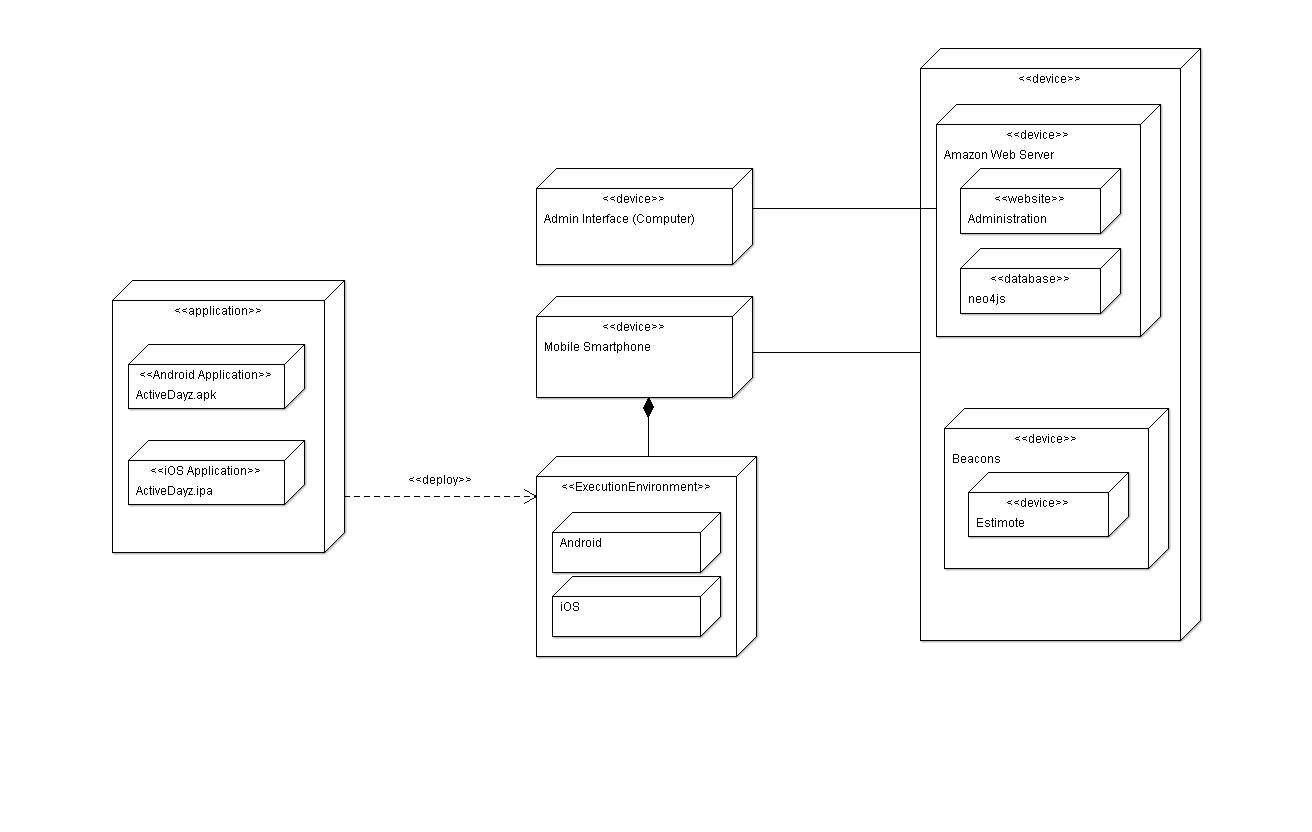
\includegraphics[width=10cm, height=8cm]{Images/DeploymentDiagram.png}\\[1cm]
\end{center}

\paragraph{Brief Description:}The Deployment diagram indicates that the application will be developed for both Android and iOS. 
These applications will then be deployed in their respective execution environments, namely: Android and iOS.
These operating systems will be run on mobile smartphones and will interact with the database to fetch location data as well as Estimote beacons in order to update current locations.
An admin interface (a computer) will then have access to an administration site to manage partners.
The database and administration site will be hosted by Amazon Cloud Services on the Amazon Web Server.

\subsection{Development Methodology}
We will be utilising \textbf{Agile} development methodologies with specific reference to \textbf{SCRUM} practices. We believe that this is the best means to enable both us as the engineering team and the client to focus on effectively performing the tasks integral to successfully providing the desired mobile application
For this project, Multiply will take the part of \emph{Product Owner} and us as Panda Inc will be the \emph{Development Team}. Subsection 3 can be seen as rudimentary version of the \emph{Product Backlog} (which will be further refined/improved in the event of this tender being accepted).
\newline \newline
Interactions are highly valued by our team, hence we are dedicated to conducting weekly or bi-weekly meetings with Multiply. This will serve and start and end points for \emph{Sprints} (which serve as schedules for delivery of agreed upon requirements) . We will also be regularly meeting and consulting with our lectures and tutors for further guidance throughout the duration of the project. All of the above mentioned parties will have access a third party instant messaging platform in order to facilitate communication apart from physical meetings. Our team will be conducting bi-daily \emph{SCRUM meetings} in order to exchange our progress statuses and to ensure an comprehensive mutual understanding is maintained
\newline \newline
A collaborative and cooperative approach between both stakeholders will be employed for the life span of the project. There will also be a focus on the frequent, iterative presentation of small, incremental releases of deliverables to the client. The \textbf{role} of Multiply in this approach includes:
\begin{itemize}
\item Active involvement and collaboration in all phases of project
  \begin{itemize}
  \item Analysis and Design - The client will facilitate the identification, definition, prioritisation and continuous refinement of high level requirements, system architecture and design decisions of the mobile application in order to ensure the correct functionality of the end product.
  \item Development and Deployment - The client will periodically review all instances of the product in order to ensure to it is in line with their expectations 
  \end{itemize}
\item Critical and constructive analysis on not only what we as the engineering team deliver but also on the quality of our service and whether or not we conducted ourselves as would be expected from those in a occupational environment
\item To provide us with the means to produce an effective end product. An exhaustive list of these required means will be provided in further Analysis and Design specification.
  
\end{itemize}
\begin{center}
{\fontfamily{UWR Grotesk}\sffamily\bfseries
\large Thank You Momentum. We at Panda Inc. look forward to working with you in the near future.
}
\end{center}

\end{document}
